\section{Differences in MAPseq output}\label{results_MAPseq_inconsistency}
During the development of the ported pipeline, the tool MAPseq was discovered to be inconsistent. Executed several times using the identical command, configuration, input, and database files, the output would occasionally vary.\par
To demonstrate this behaviour MAPseq was executed ten times, in conjunction with the MGnify-compatible database files and the SSU FASTA file from analysis MGYA00578954 (\Cref{tab:soil-samples}) as an input. Subsequently, each output was compared to the MGnify output using beta diversity metrics, specifically Bray Curtis distance and Jaccard distance, as previously described in \Cref{sec:Benchmark}.

\begin{figure}[H]
  \centering
  \hfill
  \subfloat{{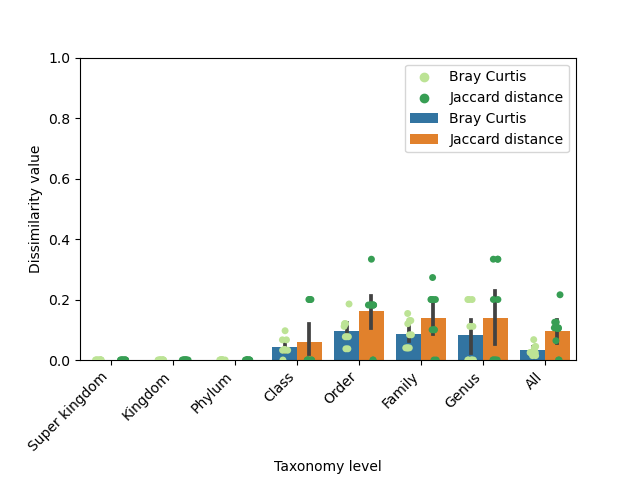
\includegraphics[scale=0.8]{figures/mapseq_test_beta_div_plot.png} }}%
  \captionof{figure}[Beta diversity-based benchmark. Dissimilarity between MGnify and MAPseq, for MAPseq inconsistency demonstration]{\textbf{Beta diversity-based benchmark}. Dissimilarity between MGnify and MAPseq. Executed ten times using identical configuration and the same sample from analysis MGYA00578954 (\Cref{tab:soil-samples}) to demonstrate MAPseq inconsistency. The term 'All' refers to all ranks combined. Species rank was excluded, due to taxa absence at this rank. Bars represent the average dissimilarity values, while individual data points represent the values for each of the ten different runs.} \label{fig:mapseq_test_beta_div_plot.png}%
\end{figure}

The dissimilarity values for MAPseq using identical input multiple times are shown in \Cref{fig:mapseq_test_beta_div_plot.png}. Neither of the execution delivered taxa in the species rank. The ranks super kingdom, kingdom, and phylum consisted of identical results. The average dissimilarity values were variable between the ranks class and genus, with the rank order having the highest average distance values for both Bray Curtis and Jaccard metrics.